\documentclass{report}
%\usepackage[utf8]{inputenc}
\usepackage{fontspec} 
\setmainfont{Bookman Old Style} % Times New Roman 
\setsansfont{Tahoma}
\setmonofont{Comic Mono}  
%\setmathfont{Latin Modern Math}
\usepackage[fontsize = 12pt]{fontsize} 
\usepackage{microtype} % added
\usepackage[english, ukrainian]{babel}
\usepackage[
    top = 40pt,
    bottom = 20pt,
    right = 50pt,
    left = 50pt,
    footskip = 15pt,
    %showframe
]{geometry}
\usepackage{amsthm}
\usepackage{amsfonts}
\usepackage{graphicx}
\usepackage[ruled]{algorithm2e}
\usepackage[unicode,
bookmarks = true,
]{hyperref} % edited
\hypersetup{
    colorlinks = true, % edited
    linkcolor = [RGB]{255, 3, 209},
    breaklinks = true,	
    filecolor = magenta,
    citecolor = green,
    anchorcolor = black,
    urlcolor = cyan,
}
\usepackage{biblatex}
\usepackage{csquotes}
\usepackage{mathtools} % {amsmath} already included here
\usepackage{amssymb}
\usepackage{enumitem} % added
\usepackage{nicefrac} % added
\usepackage{tabularray} % added
\usepackage[x11names]{xcolor}
\usepackage{tikz}
\usetikzlibrary{patterns.meta} % added
\usetikzlibrary{decorations.pathmorphing}
\usetikzlibrary {arrows.meta} % added
\usetikzlibrary{calc} % added
\usetikzlibrary{shapes.geometric} % added
\usetikzlibrary{intersections}  % added
\usepackage{pgfplots} % added
\usepackage{pgfplotstable} % added
\pgfplotsset{compat=newest} % added
\usetikzlibrary{pgfplots.fillbetween} % added
\pgfdeclarelayer{pre main} % added
\usepackage{xparse} % added for using \NewDocumentCommand (but not necessary)
\usepackage{rotating} % added
\usepackage{diagbox} % added
\usepackage[center]{caption} % added
\usepackage[warnings-off={mathtools-colon,mathtools-overbracket}]{unicode-math} % added
\usepackage{multirow} % added
\usepackage{fancyhdr} % added
\usepackage[absolute,overlay]{textpos} % added

\begin{document}
\thispagestyle{empty}
\linespread{1.1}

\begin{center}
    {\bfseries\large
        НАЦІОНАЛЬНИЙ ТЕХНІЧНИЙ УНІВЕРСИТЕТ УКРАЇНИ \\
        <<КИЇВСЬКИЙ ПОЛІТЕХНІЧНИЙ ІНСТИТУТ \\
        імені Ігоря СІКОРСЬКОГО>> \\
        Навчально-науковий фізико-технічний інститут \\
        \medskip
        Кафедра математичних методів захисту інформації}
\end{center}

\begin{center}
\vspace{40mm}
{\bfseries\huge Звіт до} \\
{\bfseries\Large комп'ютерного практикуму \No 1} \\
\end{center}

\vspace{55mm}
\begin{center}
    \hfill
    \begin{minipage}[t]{0.4\textwidth}
        \begin{flushright}
            \textbf{Оформлення звіту:} \\ 
            Дигас Богдан, ФІ-52мн \\
            Юрчук Олексій, ФІ-52мн 
        \end{flushright}
    \end{minipage}
\end{center}

\vfill
\begin{center}
    \today \\
    {м. Київ}
\end{center}

\newpage
\pagenumbering{gobble}

\renewcommand{\chaptername}{Комп'ютерний практикум \No}
\makeatletter
\renewcommand{\@pnumwidth}{2em}
\renewcommand{\@tocrmarg}{3em}
\makeatother

\cleardoublepage
\pagenumbering{arabic}
\setcounter{page}{1}
\newpage

% Clear the header and footer
\fancyhead{}
\fancyfoot{}
% Set the right side of the footer to be the page number
\renewcommand{\headrulewidth}{0pt}
\renewcommand{\footrulewidth}{0pt}
\fancyfoot[C]{
  \begin{textblock*}{2cm}(20cm,27.3cm) % bottom right corner of A4
    \small\thepage
  \end{textblock*}
}
\pagestyle{fancy}


\theoremstyle{plain}
\newtheorem{definition}{Означення}%[section]
\newtheorem{theorem}{Теорема}[chapter]
\newtheorem{claim}{Твердження}[chapter]

\theoremstyle{definition}
\newtheorem*{remark}{Зауваження:}
\newtheorem*{example}{Приклад}
\newtheorem{lemma}{Лема}[chapter] 

\renewcommand*{\proofname}{Доведення:} 

\NewDocumentCommand{\MakeWaveComment}{m}{
  \ifmmode % if math mode, make indent before bigger
    \hspace{3pt}
  \fi
  \tikz[baseline={(textnode.base)}]{
    \draw[decorate, decoration={snake, segment length=0.35cm, amplitude=1.5pt}] % Left wave line
    (0,0) -- ++(0,1.5);
    
    \node[anchor=base west, inner sep = 0.5pt] (textnode) at (0.15,0.75) {#1}; % Text node
    
    \draw[decorate, decoration={snake, segment length=0.35cm, amplitude=1.5pt}] % Right wave line
    ([xshift=0.2cm, yshift=-0.75cm]textnode.east) -- ++(0,1.5);
  }
  \ifmmode % if math mode, make indent after bigger
    \hspace{3pt}
  \fi
}

\NewDocumentCommand{\inbuildRef}{mm}{  
  \hyperref[{#1}]{#2}
}

\noindent\textbf{Мета роботи:} Ознайомлення з принципами баєсівського підходу в криптоаналізі, побудова детерміністичної та стохастичної 
вирішуючих функцій для моделей схем шифрування та криптоаналіз моделей шифрів за допомогою програмної реалізації, зокрема здійснення 
порвіняльного аналізу вирішуючих функцій.

\noindent\textbf{Постановка задачі:}
\begin{enumerate}
    \item Створіть репозиторій у системі контролю версій Git/GitHub;
    \item Реалізуйте алгоритми програмно та представите результати побудови детермінованих та стохастичних вирішальних функцій у 
        вигляді таблиць. Для цього необхідно:
        \begin{enumerate}
            \item обчислити розподіли $P(C)$ та $P(M, C)$;
            \item на основі цих розподілів обчислити $P(M \vert C)$;
            \item побудова оптимальних детермінованих та стохастичних вирішальних функцій зводиться до максимізації $P(M \vert C)$.
        \end{enumerate}
    \item Розрахуйте середні втрати, проведіть порівняльний аналіз функцій прийняття рішень.
    \item Підготувати звіт для комп'ютерного практикуму.
\end{enumerate}

\begin{center}
    \textbf{ВАРІАНТ 15}
\end{center}
Результати виконання роботи:
\begin{figure}[!ht]
        \centering
        \begin{minipage}{\linewidth}
            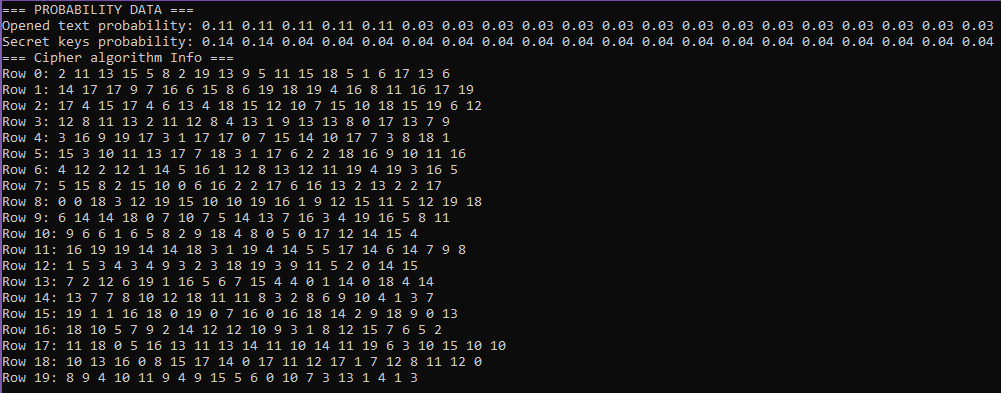
\includegraphics[width=0.8\textwidth]{/ReportPic/report_1.png}
        \end{minipage}
\end{figure}
\begin{figure}[!ht]
        \centering
        \begin{minipage}{\linewidth}
            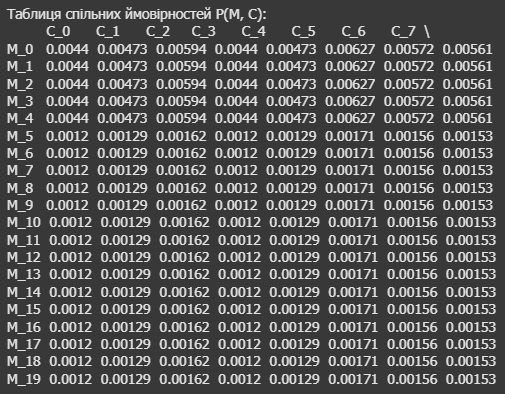
\includegraphics[width=0.4\textwidth]{/ReportPic/report_2.1.png}
        \end{minipage}
        \begin{minipage}{\linewidth}
            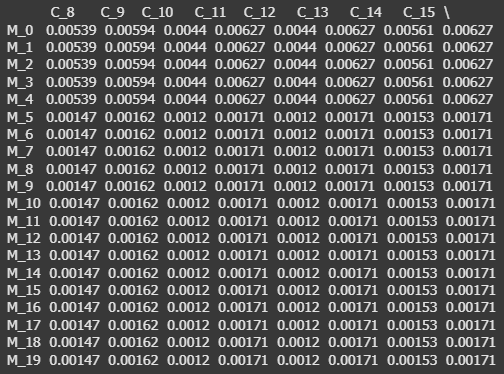
\includegraphics[width=0.4\textwidth]{/ReportPic/report_2.2.png}
        \end{minipage}
        \centering
        \begin{minipage}{\linewidth}
            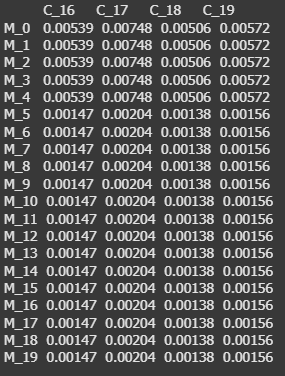
\includegraphics[width=0.15\textwidth]{/ReportPic/report_2.3.png}
        \end{minipage}
\end{figure}

Як результат роботи - видало перший ліпший $M_{i}$ (за критеріями підходить декілька)

\end{document}